\documentclass[a4paper,12pt]{article}
\usepackage{../packages/coursCollege}
\newcommand{\Chapitre}{Fonctions}
\renewcommand{\path}{../}

\usepackage[    %backend=biber,
    natbib=true,
    style=numeric,
    sorting=none]{biblatex}  % Load biblatex for bibliography handling
\addbibresource{biblio-der.bib}
\renewcommand\refname{Sources}
\renewcommand{\cours}{1MA~--~EG~--~ns~--~2025-2026}
\begin{document}
\tocloftpagestyle{fancy}
% Reduce space between section entries
\setlength{\cftbeforesecskip}{2pt}

% Reduce indentation for section entries
\setlength{\cftsecindent}{1em}

\begin{center}
	{\bfseries \Huge Fonctions}



\end{center}

\vspace{-1cm}

\tableofcontents

\newpage
\section{Généralités sur les fonctions}
\subsection{Découverte de quelques fonctions et vocabulaire}
\insertexo{n6f5f}{false}{exo}
\begin{center}
	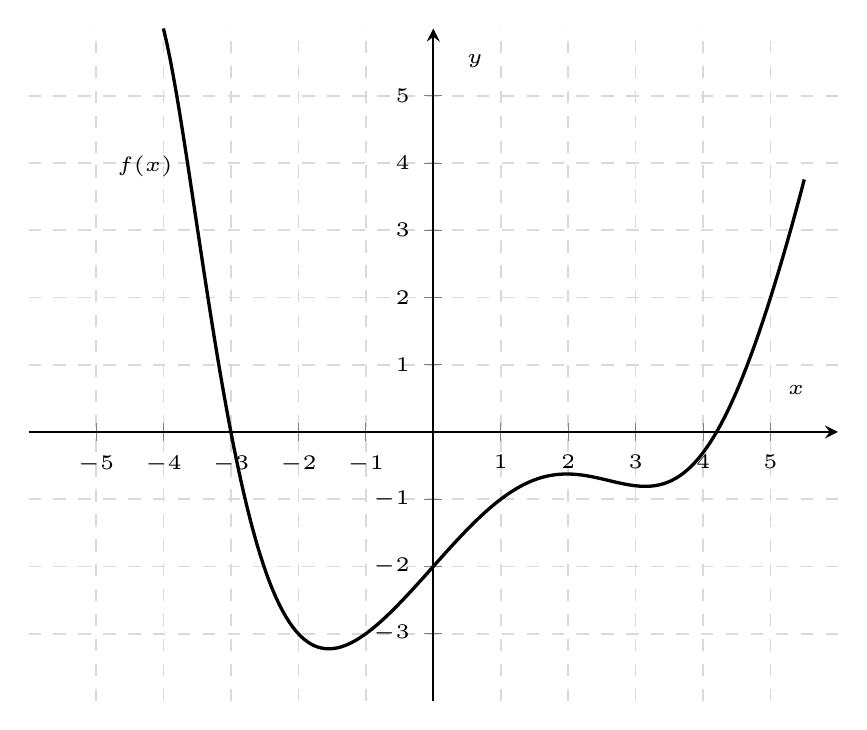
\begin{tikzpicture}[scale=1.5]
  \begin{axis}[
    axis lines=middle,
    xlabel={$x$}, ylabel={$y$},
    every axis x label/.style={at={(ticklabel* cs:0.92)}, anchor=west, yshift=10pt},
    every axis y label/.style={at={(ticklabel* cs:0.92)}, anchor=south, xshift=10pt},
    xmin=-6,   xmax=6,
    ymin=-4,   ymax=6,
    xtick={-5,-4,-3,-2,-1,0,1,2,3,4,5},
    ytick={-3,-2,-1,0,1,2,3,4,5},
    grid=both,
    grid style={dashed,gray!30},
    tick label style={font=\tiny},
    xlabel style={font=\tiny},
    ylabel style={font=\tiny}
  ]
    % branche pour x > 9
    \addplot[domain=-4:5.5, samples=200, thick]
      {-2 + 1.12406*x - 0.0055405*x^2 - 0.120957*x^3 + 0.00248144*x^4 - 0.00311538*x^5 + 0.003193*x^6 + 0.00000448489*x^7 - 0.000133948 *x^8 + 0.0000122393*x^9
}
      node[left,pos=0.1, font=\tiny] {$f(x)$};
  \end{axis}
\end{tikzpicture}
\end{center}

\insertexo{b6cb8}{false}{exo}
\insertexo{b2603}{false}{exo}
\insertexo{lfcbb}{false}{exo}
\insertexo{z0962}{false}{exo}
\insertexo{v54f9}{false}{exo}
\insertexo{cb3da}{false}{exo}
\insertexo{c1e38}{false}{exo}
\insertexo{f8be0}{false}{exo}
\insertexo{u3450}{false}{exo}
\insertexo{i705d}{false}{exo}
\subsection{Domaine de définition}
\insertexo{cd938}{false}{exo}
\insertexo{m167b}{false}{exo}
\insertexo{q7bcb}{false}{exo}
\insertexo{v3d78}{false}{exo}
\insertexo{k0236}{false}{exo}
\insertexo{h4652}{false}{exo}
\insertexo{u1722}{false}{exo}
\subsection{Opérations sur les fonctions}
\insertexo{d7ab2}{false}{exo}
\insertexo{tcbf7}{false}{exo}
\subsection{Composition de fonctions}
\insertexo{f6d6b}{false}{exo}
\insertexo{s13bb}{false}{exo}
\insertexo{k33be}{false}{exo}
\insertexo{je439}{false}{exo}
\insertexo{jd7da}{false}{exo}
\insertexo{c688a}{false}{exo}
\insertexo{k3146}{false}{exo}
\insertexo{f02af}{false}{exo}
\insertexo{l5835}{false}{exo}
\insertexo{v91bb}{false}{exo}
\insertexo{pbb73}{false}{exo}
\insertexo{wb9ff}{false}{exo}
\insertexo{b8eb6}{false}{exo}
\insertexo{a5561}{false}{exo}
\insertexo{ua665}{false}{exo}
\insertexo{u082f}{false}{exo}
\insertexo{o3a87}{false}{exo}
\insertexo{d775a}{false}{exo}
\insertexo{pa02f}{false}{exo}
\insertexo{fa8ff}{false}{exo}
\insertexo{t3d16}{false}{exo}
\insertexo{x1fab}{false}{exo}
\insertexo{u416d}{false}{exo}
\insertexo{of723}{false}{exo}
\insertexo{b2bfd}{false}{exo}
\insertexo{fcacb}{false}{exo}
\insertexo{u5d18}{false}{exo}
\insertexo{lc23a}{false}{exo}
\insertexo{jf835}{false}{exo}
\insertexo{t4cab}{false}{exo}
\insertexo{u06a8}{false}{exo}
\insertexo{x844f}{false}{exo}
\insertexo{jb01e}{false}{exo}
\insertexo{a2371}{false}{exo}
\insertexo{sc0ae}{false}{exo}
\insertexo{x1384}{false}{exo}
\insertexo{i34c4}{false}{exo}
\insertexo{f5f9a}{false}{exo}
\insertexo{z8537}{false}{exo}
\insertexo{cc016}{false}{exo}
\insertexo{h2451}{false}{exo}

Intersections

\insertexo{h3c4c}{false}{exo}
\insertexo{lf2a1}{false}{exo}
\insertexo{h5627}{false}{exo}
\insertexo{p5deb}{false}{exo}
\textbf{Problèmes d'optimisation}
\insertexo{efc34}{false}{exo}
\insertexo{x07dc}{false}{exo}
\insertexo{x8166}{false}{exo}
\insertexo{u4adb}{false}{exo}
\insertexo{ne2ae}{false}{exo}
\insertexo{bf450}{false}{exo}

\section{Les droites}
\section{Les paraboles}
\end{document}
